\state{Reflectivity of metals}{	\label{3}
	The phase velocity of light in a conducting medium is the speed of light divided by the complex dielectric constant $\Nomg = \sqrt{\epsomg}$ where we may use for $\eps$ the Drude result
	\eqn{eps}{
		\epsomg = 1 - \frac{\omgp^2}{\omg^2 + i \omg / \tau}.
	}
	In a good Drude metal, we have $1 / \tau \ll \omgp$.
}

\prob{
	Sketch curves of
	\begin{enumerate}
		\item $\Re[\sigomg]$,
		\item $\Re[\epsomg]$,
		\item $\Im[1 / \epsomg]$.
	\end{enumerate}
}

\sol{
	The conductivity is defined in (5.25) of the lecture notes:
	\eq{
		\sigomg = \frac{\omgp^2}{4\pi (1 / \tau - i \omg)}.
	}
	Thus
	\eqn{3ai}{
		\Re[\sigomg] = \frac{\omgp^2}{4\pi \tau} \frac{1}{1 / \tau^2 + \omg^2}.
	}
	Note also that
	\eqn{3aii}{
		\Re[\epsomg] = 1 - \frac{\omgp^2}{1 / \tau^2 + \omg^2}.
	}
	and that
	\eqn{3ax}{
		\Im[\epsomg] = \frac{\omgp^2}{\tau \omg} \frac{1}{1 / \tau^2 + \omg^2}.
	}
	
	Also,
	\eq{
		1 / \epsomg = \paren{ 1 - \frac{\omgp^2}{\omg^2 + i \omg / \tau} }^{-1}
		=  \paren{ \frac{\omg^2 + i \omg / \tau - \omgp^2}{\omg^2 + i \omg / \tau} }^{-1}
		= \frac{\omg^2 + i \omg / \tau}{\omg^2 + i \omg / \tau - \omgp^2}
	}
	so
	\eqn{3aiii}{
		\Im[1 / \epsomg] = \frac{(\omg / \tau) (\omg^2 - \omgp^2) - \omg^3 / \tau}{(\omg^2 - \omgp^2)^2 + \omg^2 / \tau^2}
		= -\frac{\omg}{\tau} \frac{\omgp^2}{(\omg^2 - \omgp^2)^2 + \omg^2 / \tau^2}.
	}
	Figure~\ref{3a} shows plots of $\Re[\sigomg]$~(blue), $\Re[\epsomg]$~(gold), and $\Im[1 / \epsomg]$~(green).
	
	\begin{figure}[t] \centering
		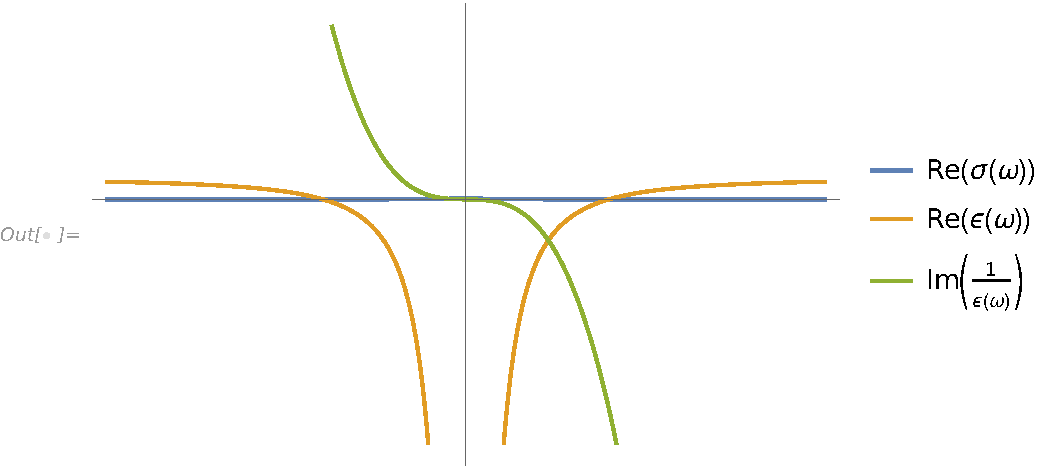
\includegraphics[width=0.49\textwidth,trim=1.5cm 0 0 0,clip]{3a} \hfill
		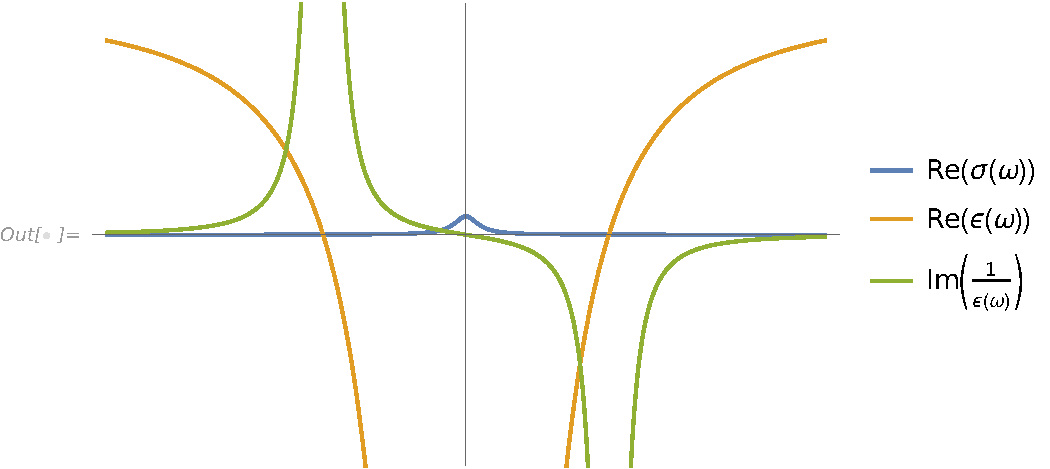
\includegraphics[width=0.49\textwidth,trim=1.5cm 0 0 0,clip]{3a2}
		\caption{Plots of $\Re[\sigomg]$~(blue), $\Re[\epsomg]$~(gold), and $\Im[1 / \epsomg]$~(green).  These expressions are given by Eqs.~\refeq{3ai}, \refeq{3aii}, and \refeq{3aiii}, respectively.  The right figure is zoomed in to show the peak in $\Re[\sigomg]$.}
		\label{3a}
	\end{figure}
}



\prob{
	Consider a light wave with the electric field polarized in the $x$ direction at normal incidence from the vacuum on a good Drude metal occupying the region $z > 0$.  In the vacuum ($z < 0$), the incident $\Eq$ and reflected $\Ew$ waves give rise to a field
	\eq{
		\Ex = \Eq e^{i \omg (z / c - t)} + \Ew e^{-i \omg (z / c + t)},
	}
	whereas in the medium, the electric field is
	\eq{
		\Ex = \Eo e^{i \omg [ \Nomg z / c - t ]}.
	}
	Matching the electric and magnetic fields on the boundary, show that
	\al{
		\Eo &= \Eq + \Ew, &
		N \Eo &= \Eq - \Ew,
	}
	and hence show that the reflection coefficient satisfies
	\eq{
		R = \abs{\frac{\Ew}{\Eq}}^2
		= \abs{\frac{1 - N}{1 + N}}^2.
	}
}

\sol{
	The magnetic fields inside and outside the medium are, respectively,
	\al{
		\By &= \frac{N}{c} \paren{ \Eq e^{i \omg (z / c - t)} - \Ew e^{-i \omg (z / c + t)} }, &
		\By &= \frac{1}{c} \Eo e^{i \omg [ \Nomg z / c - t ]},
	}
	since $v = c / N$ as stated in \ref{3}~\cite[p.~403]{Griffiths}.  The electrodynamic boundary conditions are~\cite[p.~402]{Griffiths}
	\al{
		\epsout \Eoutperp &= \epsin \Einperp, &
		\Boutperp &= \Binperp, &
		\Eoutpar &= \Einpar, &
		\frac{\Boutpar}{\muout} &= \frac{\Binpar}{\muin},
	}
	where ``in'' represents the field, permittivity, or susceptibility inside the medium and ``out'' that outside the medium.  Here, $\epsin = \epsomg$, $\epsout = 1$, and $\muin = \muout = 1$.  Since there are no components perpendicular to the surface, we only need the third and fourth equation.  By the third,
	\eqn{E1}{
		\ans{ \Eq + \Ew = \Eo }
	}
	as desired.  By the fourth,
	\eqn{E2}{
		\frac{1}{c} (\Eq - \Ew) = \frac{N}{c} \Eo
		\qimplies
		\ans{ N \Eo = \Eq - \Ew }
	}
	as we wanted to show~\cite[p.~404]{Griffiths}.
	
	Since the $\Eq$ and $\Eo$ terms of the field are propagating in the same direction, $\Eq$ must be the amplitude of the incident wave and $\Eo$ the amplitude of the transmitted wave.  The $\Ew$ component is propagating in the opposite direction, and so $\Ew$ is the amplitude of the reflected wave.  The reflection coefficient is defined by
	\eq{
		R = \frac{\IR}{\II},
	}
	where $\IR$ and $\II$ are the intensities of the reflected and incident waves, respectively.  The intensity is defined by~\cite[p.~402]{Griffiths}
	\eq{
		I = \frac{1}{2} \eps v E^2.
	}
	Thus
	\eq{
		R = \frac{\eps v \Ew^2 / 2}{\eps v \Eq^2 / 2}
		= \abs{\frac{\Ew}{\Eq}}^2.
	}
	Adding and subtracting Eq.~\refeq{E1} and \refeq{E2}, we find
	\al{
		(1 + N) \Eo &= 2 \Eq, &
		(1 - N) \Eo &= 2 \Ew.
	}
	Then
	\eqn{R}{
		R = \abs{\frac{2 \Ew}{2 \Eq}}^2
		= \abs{\frac{(1 - N) \Eo}{(1 + N) \Eo}}^2
		= \ans{ \abs{\frac{1 - N}{1 + N}}^2 }
	}
	as we wanted to show. \qed
}



\prob{
	Using the Drude formula above, show that
	\eqn{Rapprox}{
		R \approx \begin{cases}
			1 - 2 \sqrt{\dfrac{\omg}{2\pi \sigo}} & \omg \ll 1 / \tau, \\[3ex]
			1 - \dfrac{2}{\omgp \tau} & 1 / \tau \ll \omg \ll \omgp, \\[3ex]
			0 & \omgp \ll \omg,
		\end{cases}
	}
	and sketch the reflectivity $\Romg$.
}

\sol{
	From Eq.~\refeq{R}, we can write
	\eqn{R}{
		R = \abs{\frac{1 - N}{1 + N}}^2
		= \frac{(1 - \Re[N])^2 + \Im[N]^2}{(1 + \Re[N])^2 + \Im[N]^2},
	}
	where we have used Ashcroft \& Mermin~(K.6).
	
	When $\omg \ll 1 / \tau$, from Eqs.~\refeq{3ai} and \refeq{3ax},
	\al{
		\Re[\epsomg] &= 1 - \frac{\omgp^2 \tau^2}{1 + \omg^2 \tau^2}
		\approx 0, &
		\Im[\epsomg] &= \frac{\omgp^2}{\tau \omg} \frac{\tau^2}{1 + \omg^2 \tau^2}
		\approx \frac{\omgp^2 \tau}{\omg}.
	}
	Then Eq.~\refeq{R} becomes (using Mathematica)
	\eq{
		\Im[N] = \sqrt{\frac{\Im[\eps]}{2}}
		\approx \sqrt{\frac{\omgp^2 \tau}{2 \omg}} = \Re[N],
	}
	so
	\al{
		R &\approx \frac{(1 - \Re[N])^2 + \Re[N]^2}{(1 + \Re[N])^2 + \Re[N]^2} \\
		&= \frac{1 - 2 \Re[N] + 2 \Re[N]^2}{1 + 2 \Re[N] + 2 \Re[N]^2} \\
		&= \frac{1 + 2 \Re[N] + 2 \Re[N]^2 - 4 \Re[N]}{1 + 2 \Re[N] + 2 \Re[N]^2} \\
		&= 1 - \frac{4 \Re[N]}{1 + 2 \Re[N] + 2 \Re[N]^2} \\
		&= 1 - \frac{2}{\Re[N]} \\
		&= 1 - 2 \sqrt{\frac{2 \omg}{\omgp^2 \tau}} \\
		&= \ans{ 1 - 2 \sqrt{\frac{\omg}{2 \pi \sigo}} },
	}
	where we have used (5.27) in the lecture notes,
	\eq{
		\sigo = \frac{\omgp^2 \tau}{4\pi}.
	}
	and the fact that
	\eq{
		\Re[N]^2 = \frac{\omgp^2 \tau^2}{2 \omg \tau}
	}
	is very large. \qed
	
	When $1 / \tau \ll \omg \ll \omgp$,
	\al{
		\Re[\epsomg] &= 1 - \frac{\omgp^2 \tau^2}{1 + \omg^2 \tau^2}
		\approx 1 - \frac{\omgp^2}{\omg^2}
		\approx -\frac{\omgp^2}{\omg^2}, &
		\Im[\epsomg] &= \frac{\omgp^2}{\tau \omg} \frac{\tau^2}{1 + \omg^2 \tau^2}
		\approx \frac{\omgp^2}{\tau \omg^3}.
	}
	Note that $\Re[N] \ll q$.  Then we can Taylor expand Eq.~\refeq{R}:
	\eq{
		R \approx 1 - \frac{4 \Re[N]}{1 + \Im[N]^2}
	}
	\hl{What did he do??}
%	We can write $\eps = r e^{i \tht}$, where
%	\al{
%		r &= \sqrt{ \frac{\omgp^4}{\omg^4} + \frac{\omgp^4}{\tau^2 \omg^6} }, &
%		\tht &= \tan[-1]( -\frac{\omgp^2}{\tau \omg^3} \frac{\omg^2}{\omgp^2} )
%		= \tan[-1](-\frac{1}{\tau \omg})
%		\approx 0.
%	}
%	Then
%	\al{
%		\Re[N] &= \sqrt{r} \cos(\frac{\tht}{2}) \approx \sqrt{r}, &
%		\Im[N] &= \sqrt{r} \sin(\frac{\tht}{2}) \approx 0,
%	}
%	so
%	\eq{
%		R = \frac{(1 - \sqrt{r})^2}{(1 + \sqrt{r})^2}
%		= \frac{1 - 2 \sqrt{r} + r}{1 + 2 \sqrt{r} + r}
%		= \frac{1 + 2 \sqrt{r} + r - 4 \sqrt{r}}{1 + 2 \sqrt{r} + r}
%		= 1 - \frac{4 \sqrt{r}}{1 + 2 \sqrt{r} + r}
%		\approx 1 - \frac{4}{\sqrt{r}}.
%	}
%	Note that
%	\eq{
%		\sqrt{r} = \paren{ \frac{\omgp^4}{\omg^4} + \frac{\omgp^4}{\tau^2 \omg^6}  }^{1/4}
%		= \frac{\omgp}{\omg} \sqrt{1 + \frac{1}{\tau^2 \omg^2} }
%		\approx \frac{\omgp}{\omg} \paren{ 1 + \frac{1}{4 \tau^2 \omg^2} }
%		\approx 2 \omgp \tau,
%	}
%	so
%	\eq{
%		\ans{ R \approx 1 - \frac{2}{\omgp \tau} }
%	}
%	as we wanted to show. \qed
	
	When $\omgp \ll \omg$, Eq.~\refeq{eps} becomes $\epsomg \approx 1$, which implies $N = 1$, so $\Re[N] = 1$ and $\Im[N] = 0$.  Then by Eq.~\refeq{R},
	\eq{
		R \approx \frac{(1 - 1)^2 + 0}{(1 + 1)^2 + 0}
		= \frac{0}{4}
		= \ans{ 0, }
	}
	as desired. \qed

	Figure~\ref{f3c}~(left) shows the exact expression for $R$ for four different values of $\tau / \omgp$: 0.1~(blue), 1~(gold), 10~(green), and 100~(red).  Figure~\ref{f3c}~(right) compares the exact expression for $\omg \ll 1 / \tau$~(blue) and for $\omg \gg 1 / \tau$~(gold) and to the approximations for $\omg \ll 1 / \tau$~(green), $1 / \tau \ll \omg \ll \omgp$~(red), and $\omgp \ll \omg$~(violet).

	\begin{figure}[t]
		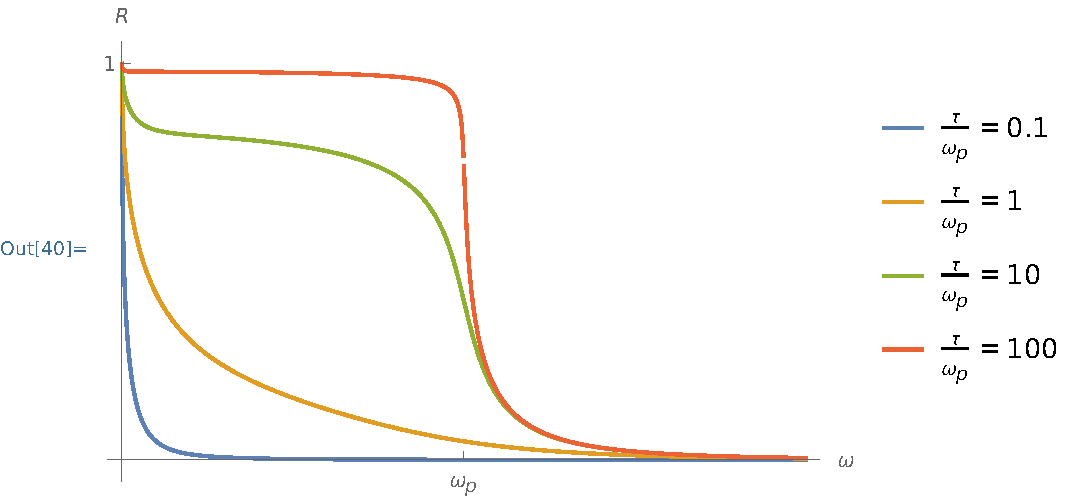
\includegraphics[width=0.49\textwidth,trim=1.5cm 0 0 0,clip]{3c} \hfill
		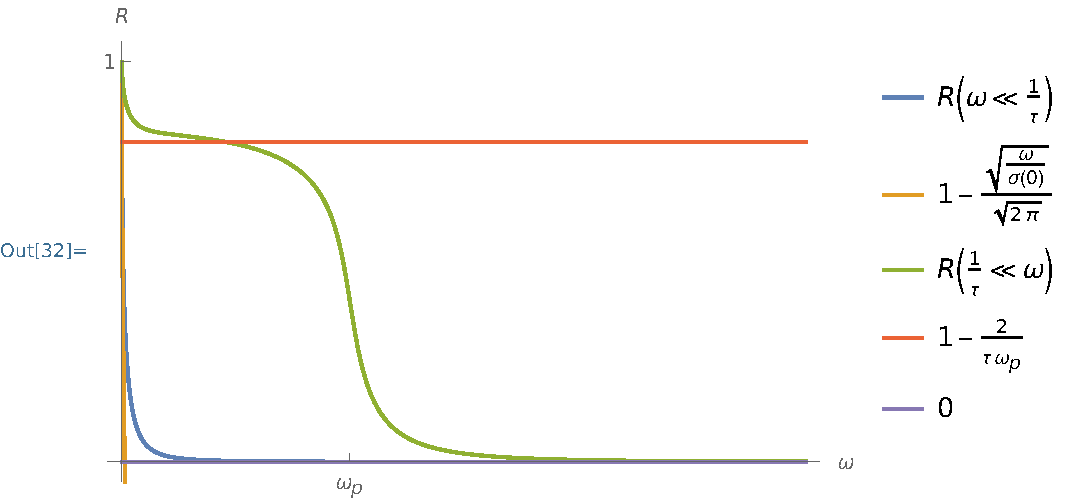
\includegraphics[width=0.49\textwidth,trim=1.5cm 0 0 0,clip]{3c2}
		\caption{Left: exact expression for $R$ in Eq.~\refeq{R} for $\tau / \omgp = 0.1$~(blue), $\tau / \omgp = 1$~(gold), $\tau / \omgp = 10$~(green), and $\tau / \omgp = 100$~(red).  Right: exact $R$ for $\omg \ll 1 / \tau$~(blue) and for $\omg \gg 1 / \tau$~(gold) and Eq.~\refeq{Rapprox} approximation for $\omg \ll 1 / \tau$~(green), $1 / \tau \ll \omg \ll \omgp$~(red), and $\omgp \ll \omg$~(violet).}
		\label{f3c}
	\end{figure}
}